\subsection{Linear SVM}
\label{fig: svmLinear}

Lets consider our training sets are given by:

\begin{equation}
  \left\{\left(\vec x_i, y_i\right)\right\}_{i=1,...,N}
  \label{eq: trainSet}
\end{equation}

where $\vec x_i = \left(x_{i1}, ... , x_{in}\right) \in \mathbb{R}^n$ are features vector in $n$-dimensional space, $y_i \in \left\{-1, 1\right\}$ defines membership to given class\footnote{$\left\{-1, 1\right\}$ was chosen for convenience in further calculations.}, $N$ is the size of training sets. A hyperplane can be defined by its normal vector ($\vec\omega = (\omega_1, ... , \omega_n)$) and an absolute term ($\omega_0$):

\begin{equation}
 \omega_0 + \underbrace{\omega_1 \cdot x_1 + ... + \omega_n\cdot x_n}_{\left<\vec\omega, \vec x\right>} = 0
 \label{eq: hyperplane}
\end{equation}

The distance ($d$) between a point $\vec x$ and a hyperplane defined by $\vec\omega$ and $\omega_0$ is given by the following formula:

\begin{equation}
 d \left(\vec x, \vec\omega, \omega_0\right) = \frac{\left|\omega_0 + \left<\vec\omega, \vec x\right>\right|}{||\vec\omega||}
 \label{eq: distance}
\end{equation}

where $||\vec\omega|| = \sqrt{\omega_1^2 + ... + \omega_n^2}$ is norm of the vector $\vec\omega$. Having that, the margin of separation ($\tau$) for training set from Eq. \ref{eq: trainSet} and a hyperplane as in Eq. \ref{eq: hyperplane} is defined as:

\begin{equation}
 \tau (\vec\omega, \omega_0) = \min_{i=1,...,N} \frac{y_i\cdot\left(\omega_0 + \left<\vec\omega, \vec x_i\right>\right)}{||\vec\omega||}
\end{equation}

so it is a distance between the hyperplane and the closest point. One should note, that absolute value from Eq. \ref{eq: distance} disappears because of smart choice of $y$ values. Points on the ``positive'' side of the hyperplane have $y = 1$, and those on the ``negative'' side have $y = -1$, which guarantees $\tau \geq 0$ (assuming all testing points are classified correctly).

\begin{figure}
 \centering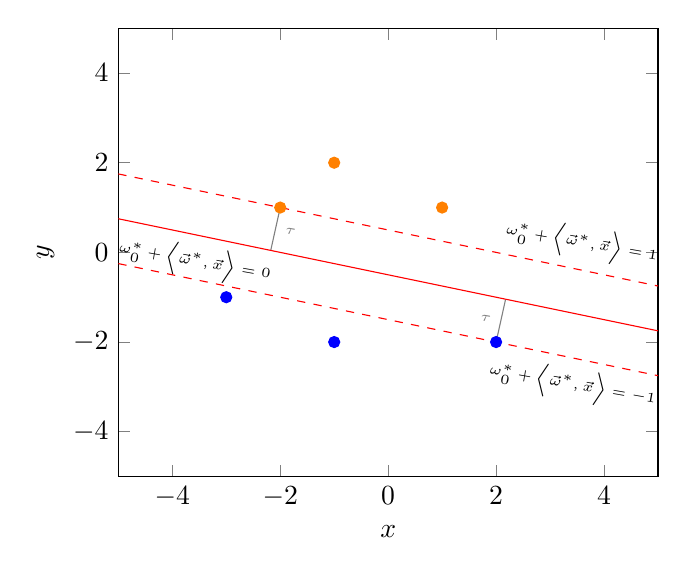
\begin{tikzpicture}

  \begin{axis}[xlabel = $x$, ylabel = $y$, xmin = -5.0, xmax = 5.0, ymin = -5.0, ymax = 5.0]
    
    \addplot[mark = *, , draw = none, color = orange] coordinates {(1,1)}; 
    \addplot[mark = *, , draw = none, color = orange] coordinates {(-1,2)}; 
    \addplot[mark = *, , draw = none, color = orange] coordinates {(-2,1)}; 

    \addplot[mark = *, , draw = none, color = blue] coordinates {(-1,-2)}; 
    \addplot[mark = *, , draw = none, color = blue] coordinates {(2,-2)}; 
    \addplot[mark = *, , draw = none, color = blue] coordinates {(-3,-1)}; 

    \addplot[mark = none, color = gray] coordinates {(-2,1) (-2.175,0.05)} node[right, pos=0.5, rotate=-10] {\tiny$\tau$}; 
    \addplot[mark = none, color = gray] coordinates {(2,-2) (2.175,-1.05)} node[left, pos=0.5, rotate=-10] {\tiny$\tau$}; 

    \addplot[color = red]         {-0.25*x - 0.5} node[below, pos=0.15, rotate=-10] {\color{black}\tiny$\omega_0^* + \left<\vec\omega^*, \vec x\right> = 0$};;
    \addplot[color = red, dashed] {-0.25*x - 1.5} node[below, pos=0.85, rotate=-10] {\color{black}\tiny$\omega_0^* + \left<\vec\omega^*, \vec x\right> = -1$};
    \addplot[color = red, dashed] {-0.25*x + 0.5} node[above, pos=0.85, rotate=-10] {\color{black}\tiny$\omega_0^* + \left<\vec\omega^*, \vec x\right> = 1$};;
    
  \end{axis}

\end{tikzpicture}
 \caption{The example of maximum-margin hyperplane separating two training sets. {\it Note, it is just a demonstrative cartoon, not real calculations.}}
 \label{fig: svmMargin}
\end{figure}

SVM is looking for the optimal hyperplane, so the one with the maximum margin of separation. The optimization task to solve is:

\begin{subequations}
 \begin{equation}
  \text{maximize}\hspace{10pt}\tau (\vec\omega, \omega_0)
 \end{equation}
 \begin{equation}
  \text{subject to}\hspace{10pt}\forall_i\hspace{5pt} y_i \cdot \left(\omega_0 + \left<\vec\omega, \vec x_i\right>\right) \geq \tau(\vec\omega, \omega_0)\cdot ||\vec\omega||
 \end{equation}
 \label{eq: optimization0}
\end{subequations}

Thus, maximize $\tau$ and make sure all points are on the right side of the hyperplane (with the distance not smaller than $\tau$). Please note, that there are still infinitively many hyperplanes fulfill these conditions (as multiplying Eq. \ref{eq: hyperplane} by a constant does not change the position of the hyperplane). One can use an arbitrary bond to determine the hyperplane unambiguously. It is convenient to use the following bond:

\begin{equation}
 \tau(\vec\omega, \omega_0)\cdot ||\vec\omega|| = 1
\end{equation}

With this bond, maximizing $\tau$ can be considered as minimizing the length of normal vector $||\vec\omega||$, so the optimization conditions from Eq. \ref{eq: optimization0} can be rewritten as:

\begin{subequations}
 \begin{equation}
  \text{minimize}\hspace{10pt} Q(\vec\omega) = \frac{1}{2}||\vec\omega||^2
  \label{eq: maximize}
 \end{equation}
 \begin{equation}
  \text{subject to}\hspace{10pt}\forall_i\hspace{5pt} y_i \cdot \left(\omega_0 + \left<\vec\omega, \vec x_i\right>\right) \geq 1
  \label{eq: condition}
 \end{equation}
 \label{eq: optimization}
\end{subequations}

where $\frac{1}{2}$ in Eq. \ref{eq: maximize} is just for convenience in further calculations. For the same reasons, the square of $||\vec\omega||$ is considered. It does not affect the final result as $||\vec\omega||$ and $Q(\vec\omega)$ have the minimum for the same $\vec\omega$. 

The example of maximum-margin hyperplane separating two training sets is presented on Fig. \ref{fig: svmMargin}, where $\omega_0^*$ and $\vec\omega^*$ denote the solution of Eq. \ref{eq: optimization}. Please note, this is just a demonstrative cartoon, not a real solution.

Eq. \ref{eq: optimization} is a quadratic programming problem. It is a kind of mathematical optimization which is extensively studied. There are many methods to solve this kind of problems. In the context of SVM Lagrange multipliers is commonly used. Sec. \ref{sec: lm} is an introduction / reminder on Lagrange multipliers. In Sec. \ref{sec: svmLinearLM} Eq. \ref{eq: optimization} is solved using this method.